\section{Homogene Differentialgleichungen 2. Ordnung}

\subsection{Einführung und Definitionen}

WIn diesem Kapitel werden wir uns mit Löung einer bestimmten Klasse von Differentialgleiuchungen befassen.

\begin{definition}{}{}
    Differentialgleichungen der Form
    \[
        \ddot{x}(t)+p\cdot\dot{x}(t)+q\cdot x(t)=0
    \]
    wobei \(p,q\in \R\) konstanten sind, heissen \emph{lineare homogene Differentialgleichungen 2. Ordnung mit konstanten Koeffizienten}
    % Eine Differentialgleichung 2. Ordnung heisst \emph{linear}, wenn sie die Form
    % \[
    %     \ddot{x}(t)+p(t)\dot{x}(t)+q(t)x(t)=r(t)
    % \]
    % hat, wobei \(p(t)\), \(q(t)\) und \(r(t)\) Funktionen von \(t\) sind.

    % Eine lineare Differentialgleichung heisst \emph{homogen}, falls
    % \(r(t)=0\) ist. Andernfalls nennt man sie \emph{inhomogen}.

    % Von einer linearen Differentialgleichung sagt man, dass sie
    % \emph{konstante Koeffizienten} besitzt, wenn die Funktionen
    % \(p(t)\) und \(q(t)\) konstant sind, also
    % \(p(t)=p\) und \(q(t)=q\).
\end{definition}

% Wir beschränken uns auf das Lösen homogener linearer Differentialgleichungen
% mit konstanten Koeffizienten, also solche der Form
% \[
%     \ddot{x}(t)+p\dot{x}(t)+qx(t)=0.
% \]

\begin{bsp}{}{}
    \begin{enumerate}
        \item \(\ddot{x}(t)+5\dot{x}(t)+6x(t)=0\)
        \item \(\ddot{x}(t)=0\)
    \end{enumerate}
\end{bsp}

Die Gleichung im zweiten Beispiel kann durch zweimaliges Integrieren
gelöst werden. Die Lösung lautet
\[
    x(t)=c_1t+c_2.
\]

Tatsächlich hat die allgemeine Lösung einer Differentialgleichung
2. Ordnung im Allgemeinen zwei frei wählbare Parameter.

\begin{satz}{Superpositionsprinzip}{}
    Seien \(x_1(t)\) und \(x_2(t)\) zwei Lösungen der Differentialgleichung
    \[
        \ddot{x}(t)+p\cdot\dot{x}(t)+q\cdot x(t)=0.
    \]
    Dann ist auch
    \[
        x(t)=c_1x_1(t)+c_2x_2(t)
    \]
    für jede Wahl von \(c_1,c_2\in\mathbb{R}\) eine Lösung
    dieser Differentialgleichung.
\end{satz}

\textbf{Beweis:}
\clearpage
\vspace{3cm}

\textbf{Bemerkungen:}

\begin{itemize}
    \item \(c_1x_1(t)+c_2x_2(t)\) nennt man eine
          \emph{Linearkombination} der Funktionen \(x_1(t)\) und \(x_2(t)\).

    \item \(x_1(t)\) und \(x_2(t)\) heissen \emph{linear unabhängig},
          falls keine der beiden Funktionen ein konstantes Vielfaches
          der anderen ist.
\end{itemize}

\begin{satz}{Allgemeine Lösung}{}
    Seien \(x_1(t)\) und \(x_2(t)\) zwei linear unabhängige Lösungen
    der Differentialgleichung
    \[
        \ddot{x}(t)+p\cdot\dot{x}(t)+q\cdot x(t)=0.
    \]
    Dann ist
    \[
        x(t)=c_1x_1(t)+c_2x_2(t)
    \]
    die allgemeine Lösung der Differentialgleichung,
    wobei \(c_1,c_2\in\mathbb{R}\) beliebige Konstanten sind.
\end{satz}

Der obige Satz reduziert das Problem des Auffindens der allgemeinen
Lösung einer Differentialgleichung 2. Ordnung auf das Ermitteln
von zwei linear unabhängigen Lösungen \(x_1(t)\) und \(x_2(t)\).
















\clearpage
\subsection{Lösungsverfahren für die Gleichung
    \texorpdfstring{\(\ddot{x}(t)+p\dot{x}(t)+qx(t)=0\)}{x''+px'+qx=0}}

\begin{LA}{}{}

    \begin{enumerate}
        \item Finden Sie die allgemeine Lösung der Gleichung
              \[
                  \ddot{x}(t)+5\dot{x}(t)+6x(t)=0.
              \]
              Tipp: Verwenden Sie den Ansatz \(x(t)=e^{\lambda t}\)
              und ermitteln Sie die möglichen Werte für \(\lambda\).
              \karofeld{5}
        \item Betrachten Sie die Gleichung
              \[
                  \ddot{x}(t)-8\dot{x}(t)+16x(t)=0.
              \]
              \begin{enumerate}
                  \item Finden Sie eine Lösung \(x_1(t)\), indem Sie
                        wie in Aufgabe 1 vorgehen.
                  \item Zeigen Sie durch Einsetzen in die Differentialgleichung,
                        dass \(x_2(t)=t\cdot e^{4t}\) auch eine Lösung ist.
                  \item Wie lautet demnach die allgemeine Lösung?
              \end{enumerate}
              \karofeld{7}
              \pagebreak
        \item Betrachten Sie die Gleichung
              \[
                  \ddot{x}(t)+x(t)=0.
              \]
              \begin{enumerate}
                  \item Gehen Sie vor wie in Aufgabe 1.
                        Wie lautet die allgemeine Lösung?
                  \item Wie muss man die Parameter \(c_1\) und \(c_2\)
                        in der allgemeinen Lösung wählen, damit daraus
                        die Lösung \(x(t)=\cos t\) resultiert?
              \end{enumerate}
              \karofeld{19}
    \end{enumerate}

\end{LA}








\pagebreak
\begin{definition}{Charakteristische Gleichung}{}
    Die Gleichung
    \[
        \lambda^2+p\lambda+q=0
    \]
    nennt man die \emph{charakteristische Gleichung} der Differentialgleichung
    \[
        \ddot{x}(t)+p\dot{x}(t)+qx(t)=0.
    \]


\end{definition}

\begin{satz}
    {}{}
    Die Funktion \(x(t)=e^{\lambda t}\) ist genau dann eine Lösung der
    Differentialgleichung, wenn \(\lambda\) eine Lösung der
    charakteristischen Gleichung ist.
\end{satz}

Um eine Differentialgleichung der Form
\[
    \ddot{x}+p\dot{x}+qx=0
\]
zu lösen, werden also zuerst die Lösungen der charakteristischen Gleichung
\[
    \lambda^2+p\lambda+q=0
\]
ermittelt. Je nach Vorzeichen der Diskriminante
\[
    D=p^2-4q
\]
dieser quadratischen Gleichung tritt einer der folgenden drei Fälle auf.

\begin{enumerate}
    \item[\textbf{1. Fall:}] \textbf{\(D>0\)}

          Die charakteristische Gleichung hat zwei verschiedene reelle Lösungen
          \[
              \lambda_1=\frac{-p+\sqrt{p^2-4q}}{2},
              \qquad
              \lambda_2=\frac{-p-\sqrt{p^2-4q}}{2}.
          \]

          Damit lösen
          \[
              x_1(t)=e^{\lambda_1t}
              \qquad\text{und}\qquad
              x_2(t)=e^{\lambda_2t}
          \]
          die gegebene Differentialgleichung.

          Da \(x_1\) und \(x_2\) linear unabhängig sind, lautet die
          allgemeine Lösung:
          \[
              \boxed{x(t)=C_1e^{\lambda_1t}+C_2e^{\lambda_2t}}
          \]

    \item[\textbf{2. Fall:}] \textbf{\(D=0\)}

          Die charakteristische Gleichung hat eine doppelte reelle Lösung
          \[
              \lambda=-\frac{p}{2}.
          \]

          Damit löst \(x_1(t)=e^{\lambda t}\) die gegebene
          Differentialgleichung.

          Ausserdem ist auch
          \[
              x_2(t)=t\,e^{\lambda t}
          \]
          eine Lösung. Um dies einzusehen, setzen wir \(x_2\) in die
          Differentialgleichung ein. Dazu benötigen wir die beiden Ableitungen:
          \begin{align*}
              \dot{x}_2(t)
               & =e^{\lambda t}+t\lambda e^{\lambda t}
              =(1+\lambda t)e^{\lambda t},             \\
              \ddot{x}_2(t)
               & =\lambda e^{\lambda t}
              +(1+\lambda t)\lambda e^{\lambda t}      \\
               & =(\lambda^2t+2\lambda)e^{\lambda t}.
          \end{align*}

          Einsetzen in die Differentialgleichung:
          \begin{align*}
              \ddot{x}_2+p\dot{x}_2+qx_2
               & =(\lambda^2t+2\lambda)e^{\lambda t}
              +p(1+\lambda t)e^{\lambda t}
              +qt e^{\lambda t}                                \\
               & =e^{\lambda t}
              \left(\lambda^2t+2\lambda+p+p\lambda t+qt\right) \\
               & =e^{\lambda t}
              \left(
              t\underbrace{(\lambda^2+p\lambda+q)}_{=0}
              +\underbrace{2\lambda+p}_{=0}
              \right)                                          \\
               & =0.
          \end{align*}

          Der erste Term ist null, weil \(\lambda\) eine Nullstelle des
          charakteristischen Polynoms ist. Der zweite ist null, weil
          \(\lambda=-\frac{p}{2}\) gilt.

          Da \(x_1\) und \(x_2\) linear unabhängig sind, lautet die
          allgemeine Lösung:
          \[
              \boxed{x(t)=C_1e^{\lambda t}+C_2t e^{\lambda t}}
          \]

    \item[\textbf{3. Fall:}] \textbf{\(D<0\)}

          Die charakteristische Gleichung hat zwei komplex konjugierte Lösungen
          \[
              \lambda=a+bi,
              \qquad
              \overline{\lambda}=a-bi,
              \qquad a,b\in\mathbb{R},\ b\neq 0.
          \]

          Damit sind
          \[
              z_1(t)=e^{\lambda t}
              \qquad\text{und}\qquad
              z_2(t)=e^{\overline{\lambda}t}
          \]
          komplexe Lösungen der Differentialgleichung.

          Die allgemeine komplexe Lösung lautet
          \[
              z(t)=C_1e^{\lambda t}+C_2e^{\overline{\lambda}t},
              \qquad C_1,C_2\in\mathbb{C}.
          \]

          In der Regel interessieren wir uns für die reellen Lösungen
          der Differentialgleichung. Bei geeigneter Wahl der Konstanten
          \(C_1,C_2\in\mathbb{C}\) lassen sich diese finden.

          Mit
          \[
              e^{i\varphi}=\cos(\varphi)+i\sin(\varphi)
          \]
          kann man die Lösungen \(z_1\) und \(z_2\) umschreiben:
          \begin{align*}
              z_1(t)
               & =e^{(a+bi)t}
              =e^{at}e^{ibt}
              =e^{at}\bigl(\cos(bt)+i\sin(bt)\bigr),    \\
              z_2(t)
               & =e^{at}\bigl(\cos(bt)-i\sin(bt)\bigr).
          \end{align*}

          Die komplexen Lösungen sind also von der Form:
          \begin{align*}
              z(t)
               & =C_1e^{at}\bigl(\cos(bt)+i\sin(bt)\bigr)
              +C_2e^{at}\bigl(\cos(bt)-i\sin(bt)\bigr)    \\
               & =(C_1+C_2)e^{at}\cos(bt)
              +(C_1-C_2)i\,e^{at}\sin(bt).
          \end{align*}

          Mit der Wahl \(C_1=C_2=\frac12\) findet man eine erste reelle Lösung:
          \[
              x_1(t)=e^{at}\cos(bt).
          \]

          Wählt man hingegen \(C_1=-\frac12 i\) und
          \(C_2=\frac12 i\), erhält man
          \[
              x_2(t)=e^{at}\sin(bt).
          \]

          Da \(x_1\) und \(x_2\) linear unabhängig sind, lautet die
          allgemeine reelle Lösung:
          \[
              \boxed{x(t)=C_1e^{at}\cos(bt)+C_2e^{at}\sin(bt)},
              \qquad C_1,C_2\in\mathbb{R}.
          \]
\end{enumerate}

\begin{satz}{Allgemeine Lösung einer homogenen linearen DGL 2. Ordnung}{}
    Seien \(\lambda_1\) und \(\lambda_2\) die Nullstellen des
    charakteristischen Polynoms zur Differentialgleichung
    \[
        \ddot{x}(t)+p\dot{x}(t)+qx(t)=0.
    \]

    Dann gilt für die allgemeine reelle Lösung der Differentialgleichung:

    \begin{enumerate}
        \item \textbf{Zwei verschiedene reelle Nullstellen:}
              \(\lambda_1\neq\lambda_2\), \(\lambda_1,\lambda_2\in\mathbb{R}\)
              \[
                  x(t)=C_1e^{\lambda_1t}+C_2e^{\lambda_2t}.
              \]

        \item \textbf{Eine doppelte reelle Nullstelle:}
              \(\lambda_1=\lambda_2=\lambda\in\mathbb{R}\)
              \[
                  x(t)=C_1e^{\lambda t}+C_2t e^{\lambda t}.
              \]

        \item \textbf{Zwei komplex konjugierte Nullstellen:}
              \(\lambda_1=a+bi\), \(\lambda_2=a-bi\),
              mit \(a,b\in\mathbb{R}\) und \(b\neq 0\)
              \[
                  x(t)=C_1e^{at}\cos(bt)+C_2e^{at}\sin(bt).
              \]
    \end{enumerate}

    Dabei sind \(C_1,C_2\in\mathbb{R}\) frei wählbare Konstanten.
\end{satz}




\clearpage
\section{Aufgaben}

\begin{ueb}{Differentialgleichungen 2. Ordnung}{}
    \begin{enumerate}
        \item Lösen Sie die folgenden Differentialgleichungen allgemein.
              \begin{enumerate}
                  \item \(\ddot{x}-4\dot{x}+4x=0\)
                  \item \(\ddot{x}+8\dot{x}+25x=0\)
                  \item \(\ddot{x}-5\dot{x}+4x=0\)
              \end{enumerate}

        \item Lösen Sie das folgende Anfangswertproblem (vgl. Aufgabe 1a):
              \[
                  \ddot{x}-4\dot{x}+4x=0,
                  \qquad x(0)=0,\quad \dot{x}(0)=1.
              \]

        \item \textbf{Federgesetz}
              \begin{center}
                  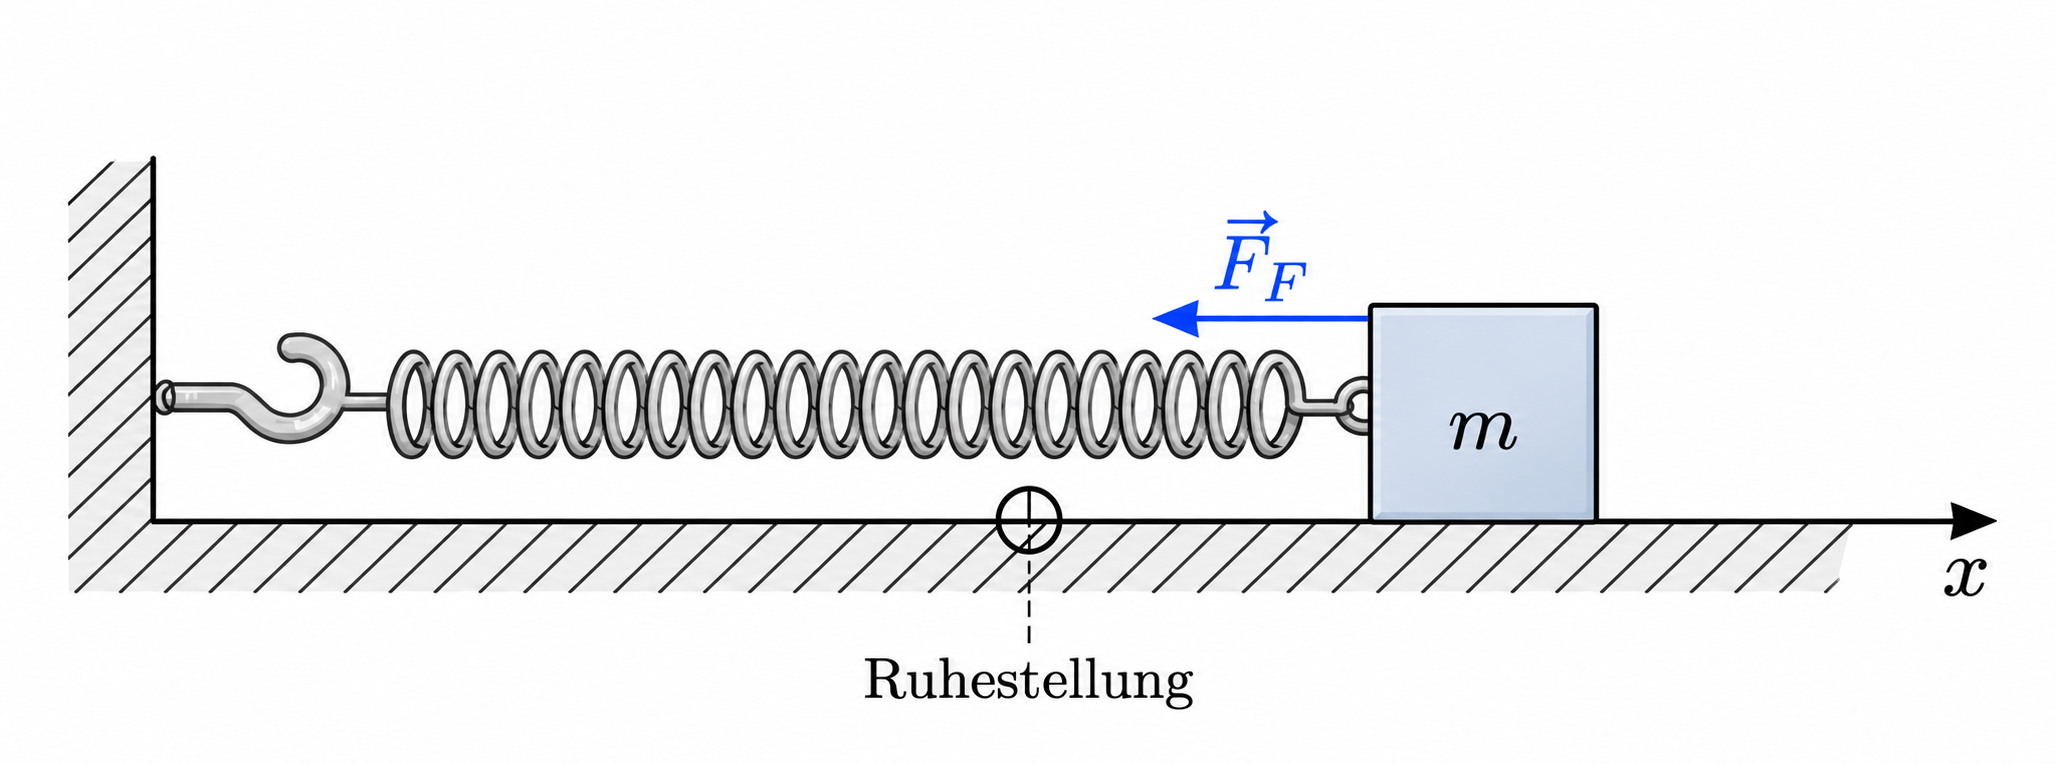
\includegraphics[width = 0.5\textwidth]{media/Technische Feder-Masse-Skizze mit Kraftvektor.png}
              \end{center}

              Nach dem Hookschen Gesetz ist die Federkraft proportional
              zur Auslenkung \(x(t)\), also
              \[
                  F_F=-k\cdot x(t).
              \]

              \begin{enumerate}
                  \item Ein Körper der Masse \(m=\SI{1}{\kilogram}\)
                        wird an eine Feder mit Federkonstante
                        \(k=\SI{4}{\newton\per\meter}\) fixiert.

                        Stellen Sie eine Differentialgleichung für \(x(t)\)
                        auf und bestimmen Sie die Lösung zu den
                        Anfangsbedingungen
                        \[
                            x(0)=5,\qquad
                            v(0)=\dot{x}(0)=0.
                        \]

                        Wie lange dauert es, bis die Masse erstmals
                        wieder beim Ausgangspunkt ist?

                  \item Ein Körper der Masse \(m=\SI{1}{\kilogram}\)
                        wird an eine Feder mit Federkonstante
                        \(k=\SI{5}{\newton\per\meter}\) fixiert.

                        Diesmal soll auch eine Gleitreibung der Form
                        \[
                            F_r=-R\cdot\dot{x}(t)
                        \]
                        mit \(R=\SI{2}{\newton\second\per\meter}\)
                        berücksichtigt werden.

                        Bestimmen Sie die Lösung der Differentialgleichung
                        zu den Anfangsbedingungen
                        \[
                            x(0)=5,\qquad
                            v(0)=\dot{x}(0)=0.
                        \]

                        Zeichnen Sie den Graphen der Lösung mit GeoGebra.
              \end{enumerate}

        \item \textbf{Kindertraum}
              \begin{center}
                  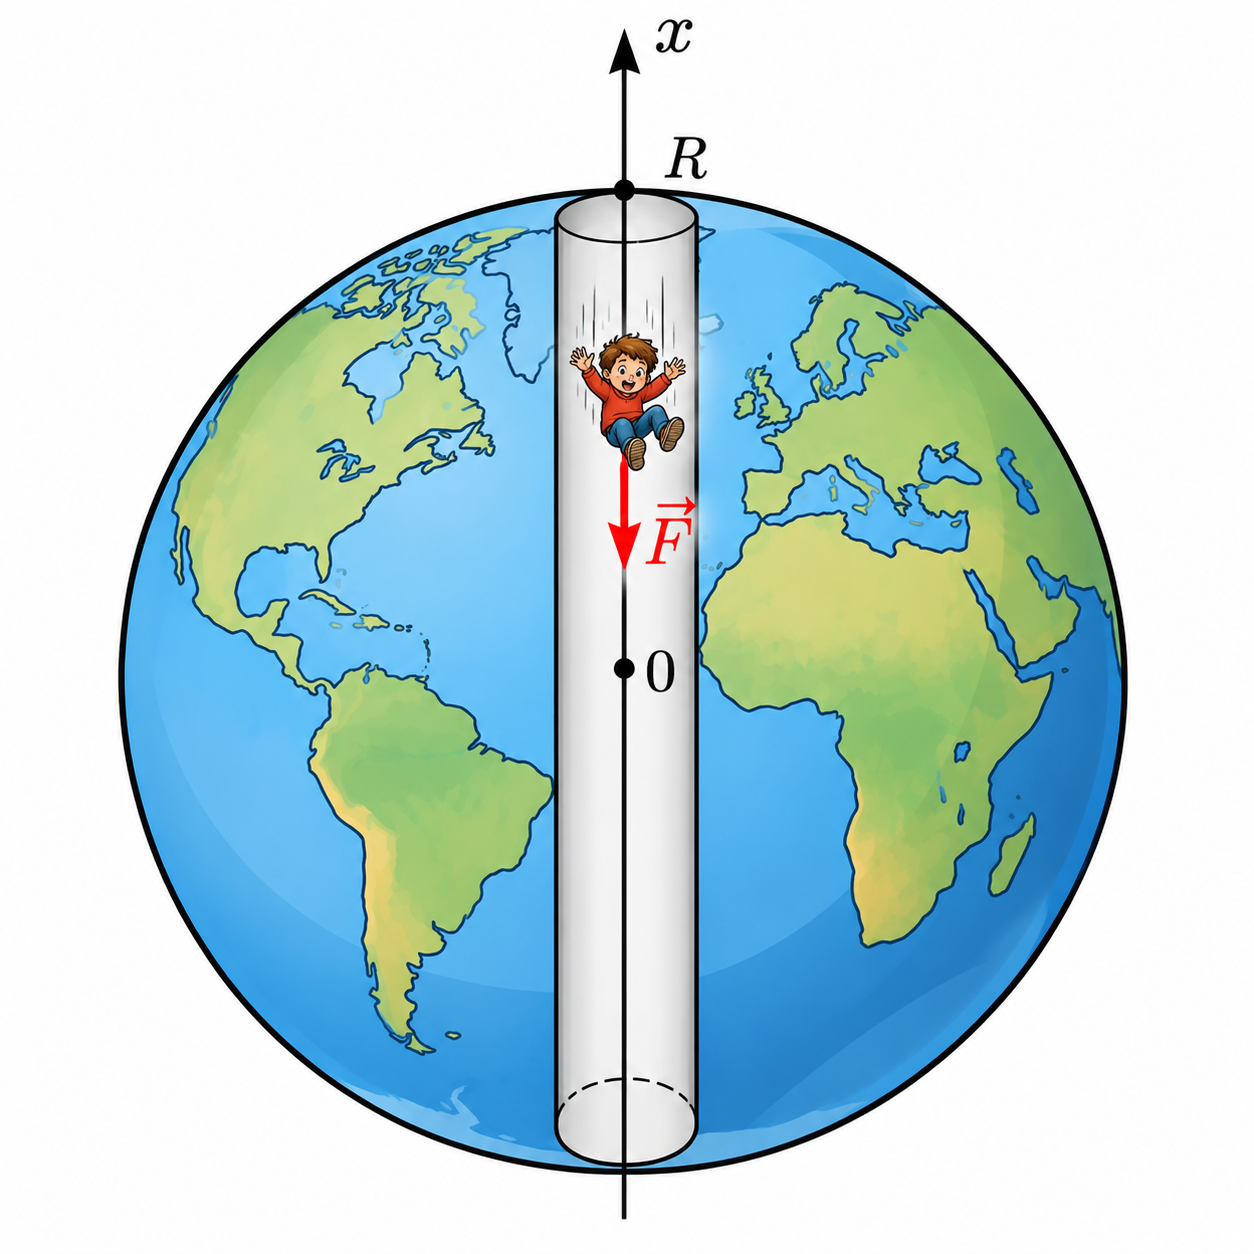
\includegraphics[width = 0.5\textwidth]{media/Physikexperiment_ Kind im Erdschacht.png}
              \end{center}

              Interessanterweise wird ein Massenpunkt der Masse \(m\)
              innerhalb einer bezüglich der Dichte homogenen Vollkugel
              der Masse \(M\) gegen die Kugelmitte hin durch eine Kraft
              angezogen, welche proportional zur Distanz \(x\) zur
              Kugelmitte abhängt:
              \[
                  F=-k\cdot x.
              \]

              Nun nehmen wir an, durch die homogene und im Inneren
              kalt vorausgesetzte Erde sei ein gerades Loch durch
              die ganze Erde gebohrt worden, welches durch die
              Kugelmitte geht.

              Was würde passieren, wenn Sie in das Loch fallen?
              (Erdradius \(R=\SI{6380}{\kilo\meter}\))

              \begin{enumerate}
                  \item Berechnen Sie die Proportionalitätskonstante
                        \(k\) in \(F=-k\cdot x\), sodass auf der
                        Oberfläche der Erde
                        \[
                            F=-m\cdot g
                        \]
                        mit \(g\approx\SI{9.81}{\meter\per\second\squared}\)
                        gilt.

                  \item Stellen Sie eine Differentialgleichung für den
                        Abstand \(x\) zum Erdmittelpunkt auf.

                  \item Lösen Sie die Differentialgleichung zu den
                        Anfangsbedingungen «reinfallen»:
                        \[
                            x(0)=R,\qquad \dot{x}(0)=0.
                        \]

                  \item Berechnen Sie die Schwingungsdauer \(T\) und
                        die maximale Geschwindigkeit \(v_{\max}\)
                        Ihrer Bewegung.
              \end{enumerate}

        \item \textbf{Ein vollkommen biegsames Seil}
              \begin{center}
                  \includegraphics[width = 0.5\textwidth]{media/Physikdiagramm_ Hängendes Seil am Tisch.png}
              \end{center}

              Ein vollkommen biegsames Seil der Länge \(l\) mit
              Masse \(m\) gleitet reibungsfrei über eine Tischkante
              gemäss Figur.

              Zum Zeitpunkt \(t=0\) wird das Seil mit der
              Anfangshöhe \(h(0)=h_0\) losgelassen
              (also \(\dot{h}(0)=0\)).

              \begin{enumerate}
                  \item Stellen Sie eine Differentialgleichung für
                        \(h(t)\) auf und bestimmen Sie die Lösung.

                  \item Berechnen Sie den Zeitpunkt \(t_{\mathrm{Ende}}\),
                        an dem das Seil die Tischkante verlässt.

                        Tipp: Verwenden Sie die hyperbolischen Funktionen
                        \[
                            \sinh(t)=\frac12(e^t-e^{-t}),
                            \qquad
                            \cosh(t)=\frac12(e^t+e^{-t}).
                        \]

                  \item Berechnen Sie für den Fall
                        \(l=\SI{1.5}{\meter}\) die Zeit
                        \(t_{\mathrm{Ende}}\) und die Geschwindigkeit
                        \(v(t_{\mathrm{Ende}})\) für die
                        Anfangsbedingung \(h_0=\SI{0.5}{\meter}\).

                        Tipp: Der Taschenrechner kennt die hyperbolischen Funktionen und deren Inversen. Dazu mussen Sie mehrmals auf die Taste \texttt{sin} bzw. \texttt{cos} drücken.
              \end{enumerate}
    \end{enumerate}
\end{ueb}

\clearpage
\textbf{Lösungen:}

\begin{enumerate}
    \item \textbf{Allgemeine Lösung}
          \begin{enumerate}
              \item \(x(t)=c_1e^{2t}+c_2te^{2t}\)

              \item \(x(t)=e^{-4t}\left(c_1\cos(3t)+c_2\sin(3t)\right)\)

              \item \(x(t)=c_1e^t+c_2e^{4t}\)
          \end{enumerate}

    \item \textbf{Anfangswertproblem}

          \[
              x(t)=te^{2t}
          \]

    \item \textbf{Feder}
          \begin{enumerate}
              \item Mit \(F=m\ddot{x}\) folgt
                    \[
                        \ddot{x}+4x=0.
                    \]
                    Die allgemeine Lösung lautet
                    \[
                        x(t)=c_1\cos(2t)+c_2\sin(2t).
                    \]
                    Aus den Anfangsbedingungen folgt
                    \[
                        x(0)=5 \Rightarrow c_1=5,
                        \qquad
                        \dot{x}(0)=0 \Rightarrow c_2=0.
                    \]
                    Somit
                    \[
                        \boxed{x(t)=5\cos(2t)}
                    \]
                    Die Masse erreicht den Ausgangspunkt erstmals wieder
                    nach einer Schwingungsdauer:
                    \[
                        T=\frac{2\pi}{2}=\pi\,\mathrm{s}.
                    \]

              \item Mit \(F=m\ddot{x}\) folgt
                    \[
                        \ddot{x}+2\dot{x}+5x=0.
                    \]
                    Die charakteristische Gleichung besitzt die Lösungen
                    \[
                        \lambda_{1,2}=-1\pm 2i.
                    \]
                    Damit lautet die allgemeine Lösung
                    \[
                        x(t)=e^{-t}
                        \left(c_1\cos(2t)+c_2\sin(2t)\right).
                    \]
                    Aus den Anfangsbedingungen folgt
                    \[
                        x(0)=5 \Rightarrow c_1=5,
                        \qquad
                        \dot{x}(0)=0 \Rightarrow c_2=\frac52.
                    \]
                    Somit
                    \[
                        \boxed{
                            x(t)=e^{-t}
                            \left(5\cos(2t)+\frac52\sin(2t)\right)
                        }
                    \]
          \end{enumerate}

    \item \textbf{Kindertraum}

          Sei \(R=6380\cdot 10^3\,\mathrm{m}\) der Erdradius.
          \begin{enumerate}
              \item Aus \(F=-kx\) und \(F(R)=-mg\) folgt
                    \[
                        k=\frac{mg}{R}.
                    \]

              \item Die Differentialgleichung lautet
                    \[
                        \ddot{x}+\frac{g}{R}x=0.
                    \]

              \item Mit \(x(0)=R\) und \(\dot{x}(0)=0\) folgt
                    \[
                        \boxed{
                            x(t)=R\cos\left(\sqrt{\frac{g}{R}}\,t\right)
                        }
                    \]

              \item Die Schwingungsdauer beträgt
                    \[
                        T=\frac{2\pi}{\sqrt{g/R}}
                        \approx 1.4\,\mathrm{h}.
                    \]
                    Die maximale Geschwindigkeit beträgt
                    \[
                        v_{\max}=R\sqrt{\frac{g}{R}}
                        \approx 7.91\,\mathrm{km/s}.
                    \]
          \end{enumerate}

    \item \textbf{Seil}

          \begin{enumerate}
              \item Die Differentialgleichung lautet
                    \[
                        \ddot{h}=\frac{g}{l}h.
                    \]
                    Mit \(h(0)=h_0\) und \(\dot{h}(0)=0\) folgt
                    \[
                        \boxed{
                            h(t)=h_0\cosh\left(\sqrt{\frac{g}{l}}\,t\right)
                        }
                    \]

              \item Das Seil verlässt die Tischkante, wenn \(h(t)=l\).
                    Damit folgt
                    \[
                        \boxed{
                            t_{\mathrm{Ende}}
                            =\sqrt{\frac{l}{g}}\,
                            \cosh^{-1}\left(\frac{l}{h_0}\right)
                        }
                    \]

              \item Für \(l=1.5\,\mathrm{m}\) und \(h_0=0.5\,\mathrm{m}\)
                    ergibt sich
                    \[
                        t_{\mathrm{Ende}}\approx 0.69\,\mathrm{s}.
                    \]
                    Die Geschwindigkeit beträgt
                    \[
                        v(t)=h_0\sqrt{\frac{g}{l}}
                        \sinh\left(\sqrt{\frac{g}{l}}\,t\right).
                    \]
                    Somit
                    \[
                        \boxed{
                            v(t_{\mathrm{Ende}})
                            \approx 3.63\,\mathrm{m/s}
                        }
                    \]
          \end{enumerate}
\end{enumerate}